% Chapter 3
\chapter{Métodos e Ferramentas} % Main chapter title
\label{chap:MetodosFerramentas} % For referencing the chapter elsewhere

\section{Metodologia}
\label{sec:metodologia-cap3}

A metodologia proposta para esta investigação inicia-se com a análise de um problema crítico no setor da construção: a \textbf{monitorização ineficaz da saúde e segurança dos trabalhadores em tempo real}. A partir de uma revisão sistemática da literatura, foram identificados os tipos de dados fisiológicos mais utilizados, bem como diversos modelos de aprendizagem, desde o Machine Learning tradicional até ao Deep Learning. Além disso, encontraram-se estudos análogos em diferentes contextos laborais que servem de base teórica e ponto de partida para esta investigação. Com base nestas evidências, a metodologia foi estruturada para responder aos objetivos propostos, seguindo uma lógica de desenvolvimento e validação dividida em três etapas principais:

\begin{itemize}
\item \textbf{Arquitetura e Integração do Sistema:} fase dedicada ao desenho da infraestrutura do Gémeo Digital Humano, estabelecendo o fluxo de dados desde a recolha sensorial até à integração do módulo preditivo, garantindo que o sistema suporte a monitorização contínua e a geração de alertas automáticos.
\item \textbf{Preparação e Caracterização de Dados:} etapa focada na análise dos sinais fisiológicos e na aplicação de técnicas de pré-processamento. Esta fase inclui a normalização, filtragem e segmentação temporal dos dados, bem como a extração de características fundamentais para alimentar os modelos de aprendizagem.
\item \textbf{Modelação, Avaliação e Comparação de Algoritmos:} fase final dedicada à exploração de diferentes abordagens de Machine Learning e Deep Learning. Os modelos são treinados e avaliados recorrendo a métricas adequadas para comparar a sua capacidade de generalização e viabilidade em cenários próximos do tempo real, permitindo a seleção da solução mais robusta para o contexto de alto risco.
\end{itemize}

Deste modo, todos os testes foram realizados inicialmente num ambiente controlado, o que permitiu validar algoritmos e estratégias de forma segura, utilizando dados reais de trabalhadores para garantir a fiabilidade e a validade científica dos resultados. Apenas após a obtenção de resultados satisfatórios no treino e na comparação dos melhores modelos, é que estas provas seriam consideradas para uma eventual transferência para o ambiente real. Esta abordagem progressiva e iterativa assegura a reprodutibilidade dos testes e a robustez da solução final face aos requisitos de segurança e bem-estar do trabalhador

\section{Arquitetura da Solução}
\label{sec:arquitetura}

A solução desenvolvida tem como objetivo principal monitorizar o estado fisiológico do trabalhador em tempo real, permitindo a deteção precoce de estados de fadiga, stress ou exaustão física. Este processo é suportado por uma arquitetura concebida para integrar de forma coerente a recolha de sinais biológicos, o processamento preditivo através de modelos de Inteligência Artificial e a representação virtual no contexto de um Gémeo Digital. Uma organização semelhante, embora aplicada ao acompanhamento de doentes com diabetes tipo 2, foi apresentada por Martinho et al. \cite{martinho2023coaching}. Esse trabalho é considerado aqui como antecedente metodológico para a separação entre recolha de dados, processamento inteligente e utilização da informação. A Figura \ref{fig:arquitetura} apresenta uma visão geral dos principais componentes e das interações estabelecidas entre eles.

\begin{figure}[H]
\centering
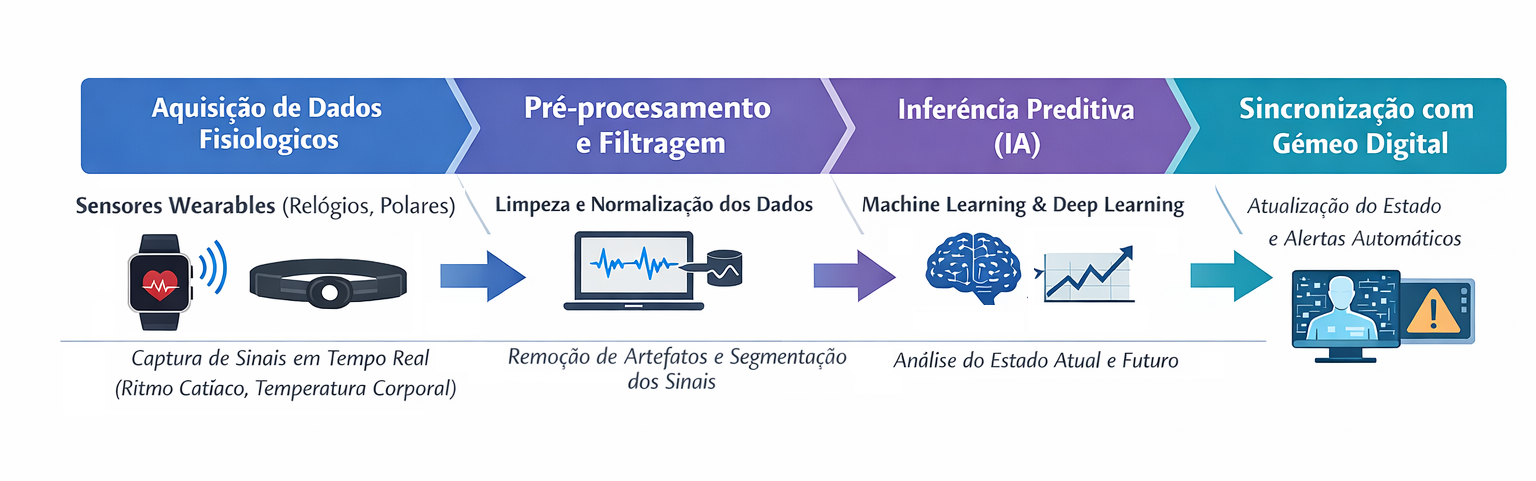
\includegraphics[width=1\textwidth]{ch3/assets/arquitectura.png}
\caption{Arquitetura da Solução}
\label{fig:arquitetura}
\end{figure}

De forma funcional, o processo pode ser descrito em quatro etapas fundamentais:

\begin{enumerate}
\item \textbf{Aquisição de Dados Fisiológicos:} os sensores wearables capturam sinais em tempo real (como ritmo cardíaco e temperatura corporal). Estes dados brutos são transmitidos para a unidade de processamento.
\item \textbf{Pré-processamento e Filtragem:} os dados recebidos são submetidos a algoritmos de limpeza para remover ruído e artefactos de movimento, sendo posteriormente normalizados e segmentados para facilitar a análise.
\item \textbf{Inferência Preditiva (IA):} os dados processados servem de entrada para os modelos de Machine Learning e Deep Learning treinados. O sistema analisa os padrões temporais para prever o estado atual e futuro do trabalhador.
\item \textbf{Sincronização com o Gémeo Digital:} Os resultados da predição e os sinais vitais são integrados na representação digital do trabalhador. Esta entidade virtual mantém o histórico e o estado atual de segurança, ativando protocolos de alerta automáticos sempre que os modelos detetem que os limiares de risco foram ultrapassados.
\end{enumerate}

Deste modo, todos os testes foram realizados inicialmente num ambiente controlado, o que permitiu validar algoritmos e estratégias de forma segura, utilizando dados reais de trabalhadores para garantir a fiabilidade e a validade científica dos resultados. Apenas após a obtenção de resultados satisfatórios no treino e na comparação dos melhores modelos, é que estas provas seriam consideradas para uma eventual transferência para o ambiente real. Esta abordagem progressiva e iterativa assegura a reprodutibilidade dos testes e a robustez da solução final face aos requisitos de segurança e bem-estar do trabalhador.

\section{Ferramentas de Hardware}
\label{sec:hardware}

Nesta secção, detalham-se os dispositivos utilizados para a recolha de dados biométricos. A escolha recaiu sobre ferramentas de elevada precisão, capazes de fornecer dados brutos (raw data) essenciais para o treino de modelos de Inteligência Artificial.

\subsection{Empatica EmbracePlus}

O \textit{Empatica EmbracePlus} \cite{empatica_embraceplus} é um smartwatch de grau médico com certificação CE Classe IIa, desenhado para a recolha contínua e passiva de dados fisiológicos em contextos de investigação e ensaios clínicos. \cite{empatica_ce_2021} O dispositivo destaca-se pela sua capacidade de fornecer métricas precisas em ambientes reais.

\subsubsection*{Sensores Integrados:}

\begin{itemize}
\item PPG (Fotopletismografia): Sensor ótico de quatro canais utilizado para a monitorização da frequência cardíaca (HR) e saturação de oxigénio (SpO2).
\item EDA (Atividade Eletrodérmica): Sensor de condutância da pele que regista a atividade do sistema nervoso autónomo.
\item Temperatura Digital: Sensor de alta precisão para o registo térmico cutâneo.
\item Acelerómetro e Giroscópio (3D): Sensores de movimento para a captura de aceleração e velocidade angular.
\item Biomarcadores Digitais Gerados: Através do processamento interno, o dispositivo gera métricas como a variabilidade da frequência cardíaca (HRV), a taxa respiratória, os níveis de intensidade de movimento e a monitorização de estados de sono e repouso.
\end{itemize}

Para além da sua capacidade sensorial, o dispositivo foi concebido para suportar as exigências físicas do trabalho de campo, conforme detalhado na Tabela \ref{tab:empatica_features}.

\begin{table}[H]
\centering
\caption{Características Físicas e Design do Empatica EmbracePlus}
\label{tab:empatica_features}
\begin{tabular}{l p{10cm}}
\hline
Característica & Descrição \\
\hline
Ecrã E-Ink & Tecnologia de tinta eletrónica always-on, que minimiza o consumo de energia e garante visibilidade ideal sob luz solar direta. \\
\hline
Robustez & Certificação IP67, garantindo resistência total a poeiras e proteção contra imersão em água. \\
\hline
Autonomia e Memória & Otimizado para gravação contínua de dados e sincronização via Bluetooth para armazenamento de longo prazo. \\
\hline
Ergonomia & Peso aproximado de 40g e bracelete de silicone hipoalergénica, desenhada para uso prolongado sem desconforto. \\
\hline
\end{tabular}
\end{table}

\subsubsection*{Fluxo de Dados e Sincronização:}

O ecossistema do relógio inteligente integra-se com a plataforma cloud \textbf{Empatica Health Monitoring Platform}. Durante a recolha ativa, o dispositivo transmite continuamente os dados biológicos para a aplicação móvel instalada no smartphone do participante através de uma ligação sem fios via Bluetooth Low Energy (BLE). Esta aplicação atua como uma ponte de comunicação intermédia, encarregando-se de sincronizar e enviar as leituras em intervalos regulares para os servidores cloud da Empatica. Através do portal online de gestão da plataforma, é possível monitorizar remotamente o funcionamento e conformidade de cada equipamento, gerir os perfis dos participantes e proceder ao descarregamento das séries temporais fisiológicas completas para posterior exportação e análise sob o formato de ficheiros CSV.

\subsubsection*{Utilização na Investigação:}

A utilização do EmbracePlus nesta investigação é fundamental, uma vez que a sua capacidade de recolha passiva de dados de Atividade Eletrodérmica (EDA), Ritmo Cardíaco (HR), Temperatura Digital, entre outros sinais fisiológicos, permite identificar biomarcadores diretamente correlacionados com estados de stress, fadiga crónica e exaustão física. Além disso, o fornecimento de métricas pré-processadas, como a Variabilidade da Frequência Cardíaca (HRV) e os níveis de intensidade de movimento, constitui uma base de dados de elevada qualidade para o treino de modelos de Inteligência Artificial. Esta robustez na aquisição de múltiplos sinais garante que os algoritmos de predição sejam treinados com dados fidedignos dos trabalhadores, permitindo fundamentar tecnicamente a antecipação de situações de risco no ambiente de construção.

\subsection{Polar H10}

O Polar H10 é um sensor de banda peitoral amplamente reconhecido na comunidade científica e desportiva pela sua precisão eletrocardiográfica (ECG). Nesta investigação, o seu uso é fundamental para validar e complementar os dados recolhidos pelo relógio, servindo como a principal referência para o estado cardiovascular do trabalhador.

\subsubsection*{Sensores e Capacidades Técnicas:}

\begin{itemize}
\item Eletrodos Pro de Alta Qualidade: Inclui elétrodos de interferência reduzida que garantem uma leitura precisa do sinal elétrico do coração, livre de artefactos de movimento.
\item Monitorização ECG: Fornece a medição da frequência cardíaca com precisão laboratorial, sendo capaz de registar cada batimento individualmente (intervalos R-R).
\item Memória Interna: Possui capacidade para armazenar uma sessão de treino completa, prevenindo a perda de dados em caso de falha na ligação Bluetooth.
\item Acelerómetro: Integra um sensor de movimento que auxilia na correção de ruído e na análise da intensidade da atividade física.
\end{itemize}

Para além da sua elevada precisão, as características físicas do Polar H10 garantem fiabilidade em condições de trabalho intensas, conforme detalhado na Tabela \ref{tab:polar_features}.

\begin{table}[H]
\centering
\caption{Características Físicas e Design do Polar H10}
\label{tab:polar_features}
\begin{tabular}{l p{10cm}}
\hline
Característica & Descrição \\
\hline
Conetividade Dual & Suporte simultâneo para Bluetooth Low Energy (BLE) e ANT+, permitindo a ligação a múltiplos dispositivos de processamento. \\
\hline
Impermeabilidade & Resistente à água até 30 metros, sendo imune ao suor intenso e a condições de chuva no ambiente de obra. \\
\hline
Autonomia & Bateria recarregável com autonomia de 20-30 horas em uso contínuo; com vida útil de até 400 horas. \\
\hline
Conforto & Banda têxtil ajustável com pontos de silicone antiderrapantes, garantindo que o sensor permanece posicionado corretamente durante o esforço físico. \\
\hline
\end{tabular}
\end{table}

\subsubsection*{Utilização na Investigação:}

A integração do Polar H10 nesta tese justifica-se pela necessidade de obter dados de frequência cardíaca com rigor médico-científico. Embora o smartwatch EmbracePlus seja o dispositivo central para a recolha multissensorial, a banda Polar H10 atua como um acompanhante fundamental devido à sua superior precisão eletrocardiográfica. Ao fornecer intervalos batimento-a-batimento (R-R) de alta fidelidade, este dispositivo permite um cálculo da Variabilidade da Frequência Cardíaca (HRV) muito mais refinado do que os sensores óticos convencionais. Esta utilização conjunta assegura uma redundância de dados que fortalece a robustez da análise, utilizando a banda como o padrão de referência para validar e elevar a confiança nas predições de fadiga e stress dos trabalhadores.
\section{Ferramentas de Software}
\label{sec:software}
O desenvolvimento desta tese e a implementação da solução tecnológica exigiram a integração de diversas ferramentas de software. Estas foram selecionadas para garantir a eficiência na gestão documental, o rigor na análise de dados fisiológicos e a robustez no treino dos modelos de Inteligência Artificial, assegurando que todo o ecossistema do Gémeo Digital Humano seja replicável e estruturado.

\subsection{Gestão de Investigação e Escrita}
Para a elaboração do documento, utilizou-se o sistema de composição tipográfica \textit{LaTeX}, baseado no motor \textit{pdfLaTeX}, que garante um padrão de elevada qualidade e rigor para documentos científicos. A edição foi realizada no \textit{Visual Studio Code} com a extensão \textit{LaTeX Workshop}, permitindo uma escrita modular dividida por capítulos e uma gestão eficiente do processo de compilação do ficheiro final em PDF.

A gestão de referências bibliográficas foi processada através do motor \textit{Biber} em conjunto com o pacote \textit{Biblatex}, assegurando a normalização automática das citações e a integridade da bibliografia ao longo de todo o trabalho. No que respeita à fundamentação teórica, a plataforma \textit{Rayyan} foi uma ferramenta determinante, servindo de suporte em todas as etapas do processo PRISMA da revisão sistemática do estado da arte (State of the Art - SoA) da investigação. Esta plataforma facilitou a triagem inicial, a exclusão de duplicados e a aplicação de critérios de inclusão e exclusão, garantindo o rigor metodológico necessário na seleção dos estudos mais relevantes para dar resposta às perguntas de investigação estabelecidas.

\subsection{Desenvolvimento Técnico e Inteligência Artificial}
No domínio técnico, o desenvolvimento foi centrado na linguagem \textit{Python}, tirando partido do seu vasto ecossistema de bibliotecas para Ciência de Dados e Inteligência Artificial. Utilizaram-se os ambientes \textit{Visual Studio Code} e \textit{Jupyter Notebook}, sendo este último fundamental para a análise exploratória, normalização de sinais e experimentação iterativa com os dados recolhidos pelo Empatica EmbracePlus e Polar H10. Para garantir a estabilidade do sistema e a reprodutibilidade dos resultados, a gestão de dependências foi efetuada através de ambientes virtuais (\textit{venv}). O controlo de versões do código foi assegurado pelo \textit{Git}, utilizando a interface \textit{GitHub Desktop} para a gestão do fluxo de trabalho e o \textit{GitHub} para o alojamento remoto, permitindo um acompanhamento detalhado de todas as fases de implementação da lógica preditiva.

\subsection{Processamento de Dados e Modelação}
O processamento dos sinais biológicos e o treino dos modelos de aprendizagem automática assentaram em bibliotecas de referência. As bibliotecas \textit{Pandas} e \textit{NumPy} foram essenciais para a manipulação de séries temporais, limpeza de ruído e alinhamento dos dados de Ritmo Cardíaco e EDA. Para a construção dos modelos preditivos de fadiga e stress, utilizou-se o \textit{Scikit-learn} em algoritmos de aprendizagem clássica e o \textit{TensorFlow} e \textit{PyTorch} para o desenvolvimento de redes neuronais. Finalmente, as visualizações estatísticas foram suportadas por bibliotecas como \textit{Matplotlib}, permitindo a tradução de dados complexos em alertas de segurança compreensíveis.

\section{Protocolo de Recolha de Dados}
\label{sec:protocolo}

A presente investigação fundamenta-se na análise de dados recolhidos no âmbito do projeto CRIARTE, um consórcio focado na colaboração entre humanos e robôs em ambientes de construção. A utilização destes dados segue um protocolo rigoroso que assegura não só a viabilidade técnica para o treino de modelos de Inteligência Artificial, mas também o cumprimento integral das normas éticas e legais vigentes.

A recolha de dados pelo projeto CRIARTE foi realizada sob o princípio da licitude, lealdade e transparência, garantindo o \textbf{consentimento informado} explícito de todos os trabalhadores participantes. Em conformidade com o Regulamento Geral sobre a Proteção de Dados (RGPD) e as diretrizes do AI Act, o protocolo adotou o princípio da minimização, assegurando que apenas os \textbf{dados estritamente necessários} para a monitorização fisiológica e segurança laboral fossem processados.

Para proteger a privacidade dos intervenientes, os dados pessoais foram sujeitos a processos de \textbf{anonimização e pseudonimização}. Esta camada de segurança garante que, embora os sinais biométricos sejam utilizados para prever estados de stress e fadiga, a identidade dos trabalhadores permanece protegida, impossibilitando a sua reidentificação direta.

Os dados foram capturados durante as jornadas reais de trabalho através dos dispositivos wearable detalhados anteriormente (Empatica EmbracePlus e Polar H10), encontrando-se organizados em ficheiros de formato Excel (.xlsx) com uma frequência de registo por minuto.

No caso do relógio EmbracePlus, o dataset consolidado inclui 22 colunas críticas para a deteção de estados emocionais e fisiológicos. Destacam-se os biomarcadores de ativação simpática como a condutância da pele (\textit{eda\_scl\_usiemens}), a frequência cardíaca basal (\textit{pulse\_rate\_bpm}) e indicadores de stress respiratório (\textit{respiratory\_rate\_brpm}). Para a análise de fadiga e recuperação, o dataset fornece a variabilidade da frequência cardíaca (\textit{prv\_rmssd\_ms}) e o gasto energético metabólico (\textit{met}). O comportamento físico é detalhado através de variáveis de movimento como activity\_counts, step\_counts e a magnitude do vetor (\textit{vector\_magnitude}), além da classificação qualitativa da atividade (\textit{activity\_class}) e da sua intensidade (\textit{activity\_intensity}), que varia entre estados sedentários e de vigor físico. Adicionalmente, o dispositivo permite monitorizar a qualidade da recuperação do trabalhador através da coluna sleep\_detection\_stage, que identifica as fases de sono (\textit{AWAKE}, \textit{LIGHT}, \textit{DEEP} e \textit{REM}).

Complementarmente, os dados provenientes da banda Polar H10 fornecem métricas de alta precisão cardiovascular, incluindo o sinal de eletrocardiograma (\textit{ECG}), frequência cardíaca (\textit{HR}) e os intervalos entre batimentos (\textit{RR}), fundamentais para validar e colmatar eventuais lacunas nos dados óticos do relógio.

Os dados brutos foram inicialmente armazenados em bases de dados seguras, seguindo as melhores práticas internacionais de integridade e segurança lógica. A gestão desta informação obedece aos princípios FAIR, garantindo que os dados sejam rastreáveis e seguros. Para os fins desta tese, o acesso a estes dados foi realizado de forma autorizada, utilizando os ficheiros consolidados que resultaram deste processo de aquisição profissional, garantindo assim uma base de dados de elevada qualidade para o treino dos algoritmos do Gémeo Digital. Estes dados serviram de base para a fase de experimentação, que compreende o pré-processamento, a engenharia de características e o treino e validação dos modelos de Inteligência Artificial, conforme detalhado no capítulo seguinte.